\documentclass[20pt]{extarticle}

\usepackage{chemfig}
\usepackage{chemmacros}
\chemsetup{modules={polymers}}
\usepackage[version=4]{mhchem}
\usepackage{graphicx}
\usepackage{hyperref}
\usepackage{IEEEtrantools}
\usepackage{textcomp}

% inkscape figures
\usepackage{import}
\usepackage{xifthen}
\usepackage{pdfpages}
\usepackage{transparent}

\graphicspath{ {./figures/} }

% labelling bonds and angles
\newcommand\namebond[5][-1pt]{\chemmove{\path(#2)--(#3)node[midway,#4,yshift=#1,black!60]{#5};}}
\newcommand\arcbetweennodes[3]{%
    \pgfmathanglebetweenpoints{\pgfpointanchor{#1}{center}}{\pgfpointanchor{#2}{center}}%
    \let#3\pgfmathresult}
\newcommand\arclabel[6][red,-stealth,shorten <=1pt,shorten >=1pt]{%
    \chemmove{%
        \arcbetweennodes{#4}{#3}\anglestart
        \arcbetweennodes{#4}{#5}\angleend
        \ifdim\anglestart pt>\angleend pt \pgfmathsetmacro\anglestart{\anglestart-360}\fi
        \draw[#1]([shift=(\anglestart:#2)]#4)arc[start angle=\anglestart,end angle=\angleend,radius=#2];%
        \pgfmathsetmacro\anglestart{(\anglestart+\angleend)/2}%
        \node[shift=(\anglestart:#2+1pt)#4,anchor=\anglestart+180,inner sep=0pt,outer sep=0pt]at(#4){#6};%
    }%
}

% for inkscape-figures
\newcommand{\incfig}[1]{%
    \def\svgwidth{\columnwidth}
    \import{./figures/}{#1.pdf_tex}
}

% more space between IEEEeqnarray lines
\begin{document}{\setlength{\IEEEnormaljot}{15pt}
% \section{Electron Configuration}
Atom's electrons go inside different shells. These shells are split into different subshells: s, p, d, and f. Each shell contains one more subshell than the one below it. That is to say, the first shell contains only the s subshell, the second shell contains the s and p subshells, the third shell contains s, p, and d, and so on. The subshells contain different numbers of orbitals
\subsection{Electron Orbitals}
An orbital can be defined as a region of space in an atom that can hold up to 2 electrons with opposite spins. The different subshells contain different numbers of orbitals.
\subsubsection{Orbitals in the s subshell}
The s subshell contains one spherical orbital. This means that the s subshell can hold up to 2 electrons
\subsubsection{Orbitals in the p subshell}
The p subshell contains three orbitals, that are lobe shaped (similar to a 3-dimensional number 8). There is one on each of the $x$, $y$, and $z$ axes. This means the p subshell can hold up to 2 electrons
\subsubsection{Orbitals in further subshells}
For A-level, knowledge of the shapes of d and f orbitals is not required. What is required is knowing that the number of orbitals keeps going up by 2. So the d subshell has 5 orbitals, and can hold up to 10 electrons. The f subshell has 7 orbitals, and can hold up to 14 electrons.

\subsection{The size of the shells}
Based on this knowledge, we can work out the sizes of all of the shells.
\begin{center}
\begin{tabular}{|c|c|c|c|c|}
\hline
Shell     & 1st Shell & 2nd Shell & 3rd Shell & 4th Shell   \\
Subshells & 1s        & 2s 2p     & 3s 3p 3d  & 4s 4p 4d 4f \\
Electrons & $2$       & $2+6$     & $2+6+10$  & $2+6+10+14$ \\
Total     & $2$       & 8         & 18        & 32          \\
\hline
\end{tabular}
\end{center}

\subsection{Writing electron configurations}
\subsubsection{Full electron configurations}
When writing out the electron configuration of an atom or ion, we write out each subshell, with the amount of electrons it contains in superscript. For example, the electron configuration of a sodium atom could be written as 1s$^2$ 2s$^2$ 2p$^6$ 3s$^1$
\subsubsection{Short form electron configurations}
If an electron configuration is extremely long, you can write it in short form. This means writing the nearest preceeding noble gas in square brackets, and then writing out just the end of the configuration. Using this, a sodium atom's electron configuration can be written as [Ne] 3s$^1$.

\subsection{Filling orbitals}
\subsubsection{Hund's rule}
Hund's rule states that each orbital in a subshell is singularly occupied before any are doubly occupied. For example, if there are 3 electrons in a p subshell, each orbital will contain just 1 electron, rather than one orbital having 2 and another 0. In addition, Hund's rule states that each of the electrons in singly occupied orbitals will have the same spin.
\subsubsection{The 4s subshell}
The 4s subshell has a lower energy than the 3d subshell, and so fills \textbf{before} the 3d subshell. Googling for ``Electron Configuration Table'' yields images which are helpful for understanding how this affects the layout of the periodic table.

% \section{Ionisation Energy}
Ionisation energy can be defined as the amount of energy required to remove 1 mole of electrons from 1 mole of gaseous particles, leaving 1 mole of gaseous ions with a more positive charge. For example:
\begin{equation}
	\ce{O^{2+}(g) -> O^{3+} + e-}
\end{equation}

\subsection{Factors affecting ionisation energy}
\subsubsection{Nuclear charge}
The overall charge of the nucleus, affected by how many protons the nucleus has. Increases down groups, and to the right of periods.
\subsubsection{Atomic radius}
How far the electrons are from the nucleus. Affected by the number of the shell containing the electron in question, and also by how many shells there are in relation to the nuclear charge (fewer shells will be held closer to a nucleus of the same positive charge, and more charge will hold the same number of shells closer).
\subsubsection{Shielding}
The amount of shielding happening because of electrons between the nucleus and the electron in question. Affected by how many shells are between the nucleus and the electron in question, as electrons on the same shell don't contribute to the shielding effect.

\subsection{Trends in first ionisation energy down groups}
Moving down groups, the nuclear charge increases. However, this increase in nuclear charge is outweighed by the increase in shielding, and increase in atomic radius, meaning that the first ionisation energy will decrease moving down groups
\subsection{Trends in first ionisation energy along periods}
In periods, as we move to the right then the nuclear charge increases, and the atomic radius decreases because the charge increased but the number of shells didn't. There is also no change to shielding because we didn't add any more shells. This means that, in general, the first ionisation energy will increase moving to the right of periods.
\subsubsection{Anomalies regarding the general trend along periods}
There are two exceptions to this general trend. That is to say, there are two points along a period will decrease rather than increase the first ionisation energy They occur at group 3 and group 6.
\\
At group 3, we go from removing the second electron from the s subshell to removing the first electron from the p subshell. The p subshell requires less energy to remove an electron from, and so the first ionisation energy is lower. For example, boron 1s$^2$ 2s$^2$ 2p$^1$ has a lower first ionisation energy than beryllium 1s$^2$ 2s$^2$, even though it is further to the right of the period.
\\
At group 6, we go from removing the third electron from the p subshell, to removing that same p subshell's fourth electron. This causes an anomaly because of Hund's rule, which states that each orbital will contain one electron before any contain two. This means that we are now removing an electron from an orbital containing two electrons, and its paired electron will repel it slightly, lowering the energy required to remove it and so again lowering the first ionisation energy. For example, oxygen 1s$^2$ 2s$^2$ 2p$^4$ has a lower first ionisation energy than nitrogen 1$^2$ 2s$^2$ 2p$^3$, even though it is further to the right of the period.

% \section{Ionic bonding}
Ionic bonds form between particles with relatively low ionisation energies, usually between metals and non-metals. If ionisation energies are high, covalent bonding will be favoured.
\subsection{How ionic bonds form}
Ionic bonds form when a metal loses electrons in order to achieve noble gas electron configuration. For example, sodium could lose one electron to form an $\ce{Na^+}$ cation. This electron is then gained by the non-metal, for example chlorine, in order to form a $\ce{Cl^-}$ anion. Electrostatic attraction between the two particles is what makes this into a bond, as the two particles are now chemically held together.

\begin{IEEEeqnarray}{C}
	\ce{Na -> Na^+ + e^-}
	\nonumber\\
	\ce{Cl + e^- -> Cl^-}
\end{IEEEeqnarray}
\begin{figure}[ht]
    \centering
    \incfig{an-ionic-bond}
	\caption{How ionic bonds are formed}
    \label{fig:an-ionic-bond}
\end{figure}

\subsection{Giant ionic lattices}
Ionic substances (as solids) are often held in giant ionic lattices. These are regular 3-dimensional lattices held together by electrostatic attraction. For the example of Sodium Chloride, each $\ce{Na^+}$ is surrounded by 6 $\ce{Cl^-}$ ions (one on each side on all 3 axes). Each $\ce{Cl^-}$ is surrounded in the same way by $\ce{Na^+}$ ions.

\subsection{Properties of ionic substances}
Melting points of ionic substances are high because of the large amount of energy required to overcome the strong electrostatic attraction between ions.
\\
Ionic substances are brittle because any dislocation causes layers to misalign, meaning that the ions will repel rather than attract, and splitting the substance.
\\
Ionic substances don't conduct electricity when solid, but do conduct when molten or when in aqueous solution. This is because the ions are free to move.
\\
Ionic substances are insoluble in non-polar solvents, but soluble in polar ones (like water). This is because polar substances are able to break down the lattice and surround each ion in solution.

% \section{Covalent Bonding}
Covalent bonds are formed between two non-metals, and based on shared pairs of electrons. That is to say, pairs of electrons are shared between atoms so that they can both gain electrons and reach noble gas electron configuration.

\subsection{How covalent bonds form}
Electrons are shared by the atoms moving together so that orbitals containing the paris of electrons overlap. The bond can be described as the attraction between a positively charged nucleus, and a shared pair of electrons.

\subsection{Representing covalent bonds}
\subsubsection{Dot and cross diagrams}
Dot and cross diagrams can be used to help us understand covalent bonds.
\begin{figure}[ht]
    \centering
    \incfig{dot-and-cross-diagram-for-h2}
	\caption{Dot and cross diagram for $\ce{H2}$}
    \label{fig:dot-and-cross-diagram-for-h2}
\end{figure}
\subsubsection{When drawing molecules}
Covalent bonds can be represented by drawing solid lines between the atoms' symbols. The number of lines represents how many pairs of electrons are shared. Each line is one shared pair of electrons. For example, ethene can be drawn like this:\\
\chemfig{C (-[3]H) (-[5]H) = C (-[1]H) (-[7]H)}

\subsection{Different kinds of electron pair}
A pair of electrons involved in a covalent bond is called a \textbf{bonding pair}. A pair of electrons not involved in a covalent bond (but in a covalently bonded molecule) is called a \textbf{lone pair}, and may be represented by a double dot when drawing molecules. For example a diagram of, $\ce{NH3}$ might be drawn something like this:
\chemfig{\lewis{2:,N} (-[4]H) (-[6]H) (-[8]H)}

\subsection{Properties of covalently bonded substances}
Covalent substances don't conduct electricity because they have no mobile ions or electrons.
\\
Covalent substances tend to be more soluble in organic solvents than in water; some are hydrolysed.
\\
Boiling points in covalent substances are low because intermolecular forces are weak, and so little energy is required to separate molecules from each other. Boiling points increase as the molecules get a larger surface area. An example would be the alkanes getting higher boiling points as chains get longer.

\subsection{Not needing NGEC}
As long as the middle atom maximises the number of covalent bonds it has, the compount will be stable. For example, in $\ce{BF3}$, boron only has 6 electrons in its outer shell, but because it has 3 covalent bonds then the molecule is stable.
\subsection{Expanding the octet (going beyond 8 electrons)}
For elements further down the periodic table, more than 4 covalent bonds can be formed. This is because the n$=3$ shell can hold 18 electrons, and so more are available for bonding, for example in phosphorus pentachloride ($\ce{PCl5}$).
\subsubsection{What's really going on (NOT IN THE SPEC)}
The phosphorus has the configuration [Ne]3s$^2$3p$^3$, with the 3s electrons being paired and the 3p electrons being unpaired (because of hund's rule). What happens is that one of the 3s electrons moves to the first 3d orbital, meaning that there are 5 electrons in the outer shell, all unpaired. This means that there can be 5 covalent bonds formed. This is known as hybridisation. In this example, the hybridisation has created the sp$^3$d hybrid orbitals (5 hybrid orbitals in total).


\subsection{Dative covalent bonds (or coordinate bonds)}
Dative covalent bonds are slightly different from covalent bonds in their formation. The shared electrons making up the bonding pair are both from one donor atom, rather than one being from each of the two that are sharing. For example, $\ce{NH4+}$ ions are formed by the lone pair from an $\ce{NH3}$ molecule being donated to an $\ce{H^+}$ ion. This can be displayed as an arrow, like this:\\
\[\chemfig{N (-[0,,,,->]H^+) (-[2]H) (-[4]H) (-[6]H)}\]$^+$

% \section{Shapes of molecules and ions}
\subsection{Electron repulsion theory}
As electrons are all negatively charged, electron pairs will repel each other. This means that bonding electron pairs will arrange themselves as far apart as possible.

\subsection{Drawing bonds in 3 dimensions}
When drawing bonds, different symbols can be used to represent bonds. A solid (\chemfig{-}) means that the bond is in line with the plane of the paper. A wedge (\chemfig{>}) means that the bond is going forward, out from the paper towards the reader. A dashed wedge (\chemfig{>:}) means that the bond is going into the paper, away from the reader.

\subsection{Shapes of molecules}
\subsubsection{Linear}
If a molecule has two bonding pairs, they will repel to be as far away from each other as possible. This is called a \textbf{linear} shape, and has angles of \textbf{180\textdegree}. An example would be beryllium chloride, and could be drawn like this:
\begin{center}
	{\chemfig{Cl-Be-Cl}}
\end{center}

\subsubsection{Trigonal planar}
If a molecule has three bonding pairs, then they will form a triangle on one plane, so that they can all be as far away as possible, This is called a \textbf{trigonal planar} shape, and has angles of \textbf{120\textdegree}. An example would be aluminium chloride and could be drawn like this: 
\begin{center}
	\chemfig{@{c}Al (-[:30]@{r}Cl) (-[:150]@{l}Cl) (-[:270]@{d}Cl)}
	\arclabel{1cm}{d}{c}{r}{\footnotesize 120\textdegree}
\end{center}
\subsubsection{Tetrahedral}
If a molecule has four bonding pairs, then they will move as far away from each other in three dimensions. The shape they form is known as \textbf{tetrahedral}, and has angles of \textbf{109.5\textdegree}. An example would be methane, which can be drawn like this:
\begin{center}
	\chemfig{@{c}C (-[:90]@{u}H) (<:[:-20]@{r}H) (<[:-80]@{d}H) (-[:199.5]@{l}H)}
	\arclabel{1.5cm}{d}{c}{r}{\footnotesize 109.5\textdegree}
\end{center}

\subsubsection{Trigonal bipyramidal}
If a molecule has five bonding pairs, then they will move as far away from each other in three dimensions forming a \textbf{trigonal bipyramidal} shape which has angles of \textbf{90\textdegree{} and 120\textdegree}. An example would be phosphorus (v) chloride, which can be drawn like this:

\begin{center}
	\chemfig{@{s}S (-[:90]@{u}F) (-[:0]@{r}F) (-[:-90]@{d}F) (<[:-135]@{ld}F) (<:[:135]@{lu}F)}
	\arclabel{1.5cm}{r}{s}{u}{\footnotesize 90\textdegree}
	\arclabel{1.5cm}{lu}{s}{ld}{\footnotesize 120\textdegree}
\end{center}

\subsubsection{Octahedral}
If a molecule has six bonding pairs, then they will move as far away from each other in three dimensions forming an \textbf{octahedral} shape which has angles of \textbf{90\textdegree}. The shape is called octahedral because that is the shape that would be formed if the ends of all the bonds were considered vertices of the shape. An example would be sulphur hexafluoride, and can be drawn like this:
\begin{center}
	\chemfig{@{s}S (-[:90]@{u}F) (-[:-90]@{d}F) (<:[:35]@{ru}F) (<:[:145]@{lu}F) (<[:-35]@{rd}F) (<[:-145]@{ld}F)}
	\arclabel{1.5cm}{ru}{s}{u}{\footnotesize 90\textdegree}
\end{center}

\subsection{Molecules with lone pairs}
Lone pairs are more electron-dense than bonding pairs, and so repel with more force, pushing more and making the molecules into irregular shapes. To determine this shape, work out how many pairs (bonded or lone) the molecule has in total. The molecule's shape will be based of the corresponding regular shape, but changed based on how many of the pairs are lone pairs.

\subsubsection{Lone pair shapes with four total pairs}
If there are four total pairs, the molecule's shape will be based on the tetrahedral shape, but with the bond angles decreased by 2.5 degrees for every lone pair. These shapes are called \textbf{pyramidal}, or sometimes trigonal pyramidal (with one lone pair), and \textbf{angular} (with two lone pairs). Examples would be ammonia and water.

\begin{center}
	\chemfig{@{n}\lewis{2:,N} (<:[:-15]@{r}H) (<[:-85]@{d}H) (-[:-170]@{l}H)}
	\arclabel{1.5cm}{d}{n}{r}{\footnotesize 107\textdegree}
\end{center}
\begin{center}
	\chemfig{@{o}\lewis{1:3:,O} (-[:-37.75]@{r}H) (-[:-142.25]@{l}H)}
	\arclabel{1cm}{l}{o}{r}{\footnotesize 104.5\textdegree}
\end{center}

\subsubsection{Lone pair shapes with six total pairs}
If there are two lone pairs and six total pairs, then the lone pairs will repel more and end up as far away from each other. This forms what is called a \textbf{square planar} shape, for example found in xenon tetrafluoride:

\begin{center}
	\chemfig{@{xe}\lewis{2:6:,Xe} (<:[1]@{ru}F) (<:[3]@{lu}F) (<[5]@{ld}F) (<[7]@{ld}F)}
	\arclabel{1.5cm}{rd}{xe}{ru}{\footnotesize 90\textdegree}
\end{center}

\subsection{Ions}
Ions work in the same way as molecules. For example, ammonium ions have a tetrahedral shape.

\subsection{Double bonds}
Double bonds are treated as bonded regions. For example, in carbon dioxide then there are two double bonds, and so two bonded regions, making the shape linear:

\begin{center}
	\chemfig{O=C=O}
\end{center}

Bonded regions are treated in exactly the same way as bonded pairs. So, by this logic a sulphate (vi) ion has a tetrahedral shape:

\begin{center}
	\chemfig{@{s}S (=[2]@{u}O) (=[:199.5]@{l}O) (<[7]@{d}\ce{O-}) (<:[:-10]@{r}\ce{O-})}
	\arclabel{1.5cm}{r}{s}{u}{\footnotesize 109.5\textdegree}
\end{center}

% \section{Electronegativity and polarity}
Electronegativity is a measure of the tendency of an atom to attract a bonding pair of electrons in a covalent bond. It is affected by the same factors affecting ionisation energy: atomic radius, nuclear charge, and electron shielding.

\subsection{Polar covalent bonds}
When atoms have different levels of electronegativity, the more electronegative atom will pull the bonding electrons towards it. For example, in \ce{HCl}, chlorine is more electronegative than hydrogen, and so the elecrons are pulled towards it. We show this with a lowercase delta. This change in charge is called a permanent dipole.
\begin{center}
	\chemfig{\chemabove[3pt]{H}{\delta +}-\chemabove[3pt]{Cl}{\delta -}}
\end{center}

\subsection{Polarity of molecules}
If a molecule has permanent dipoles and is non-symmetrical, then the molecule is considered polar. For example, with water, then it has a permanent dipole across both of the bonds, and then are non-symmetrical, as they'd have to be vertically opposite to cancel out but the molecule has an angular shape.
\begin{center}
	\chemfig{\chemabove[3pt]{O}{\delta +}(-[-1]\chemabove[3pt]{H}{\delta -})(-[-3]\chemabove[3pt]{H}{\delta -})}
\end{center}

A different example would be tetrachloromethane, \ce{CCl4}. It has four permanent dipoles, but they cancel in the tetrahedral shape leaving a non-polar molecule.
\begin{center}
	\chemfig{
		\chemabove[3pt]{C}{\delta +}
		(-[3]\chemabove[3pt]{Cl}{\delta -})
		(-[5]\chemabove[3pt]{Cl}{\delta -})
		(<[1]\chemabove[3pt]{Cl}{\delta -})
		(<:[-1]\chemabove[3pt]{Cl}{\delta -})
	}
\end{center}

\subsection{The Pauling scale}
The Pauling scale is a scale for measuring elecronegativity. It was invented by Linus Pauling. This is important because the greater the difference in electronegativity, the greater the permanent dipole formed.

\subsection{Trends in electronegativity}
\subsubsection{To the right of periods}
Electronegativity increases to the right of periods. This is because the shielding stays the same, while the nuclear charge increases and the atomic radius decreases. This means that there's more charge pulling the pair towards the nucleus, and this is compounded by the fact that the pair will be closer to the nucleus in the first place (and so more susceptible to its attraction).
\subsection{Down groups}
Electronegativity decreases down groups. This is because the shielding increases, and the atomic radius increases. The nuclear charge increases, but not enough to counteract the increase in both shielding and atomic radius, making the overall electronegativity decrease down the group.


\section{Intermolecular forces}
Intermolecular forces influence a variety of the physical properties of substances, the most notable of which is their melting and boiling points. Also, if a substance sublimes, it is because the intermolecular forces are extremely weak. There are three types of intermolecular forces.

\subsection{London forces}
These are attractive forces which happen between temporary and induced dipoles, and happen in all molecules. Because of electron oscillation, at any given moment one side of an atom will be electronegative while the other side will be electropositive by a very small amount (as more electrons will be on one side of the molecule). This is called a temporary dipole. These temporary dipoles induce similar dipoles in the surrounding molecules, and as such the dipoles will cause the molecules to have a small electrostatic attraction. As the number of electrons increases, the strength of London forces also increases, as the number of electron oscillations increase and so it is more likely for the molecule to have a stronger temporary dipole.

\subsection{Permanent dipole-dipole interactions}
These are attractive forces that happen between permanent dipoles in polar molecules. The permanent dipole in one molecule attracts the permanent dipole fo another. Substances that have permanent dipole-dipole interactions often have higher boiling points than those that don't as there is extra energy required to overcome them.

\subsection{Van der Waal's forces}
This is an old term that just refers to both London forces, and also to permanent dipole-dipole interactions.

\subsection{Hydrogen bonding}
This is a strong intermolecular force, that happens in covalent molecules which have extremely electronegative atoms (O, N, or F) with lone pairs, and also hydrogens. The interactions happen between the $\delta^+$ at the hydrogens, and the lone pairs of the electronegative atoms in other molecules. An example would be water.
\begin{figure}[h]
	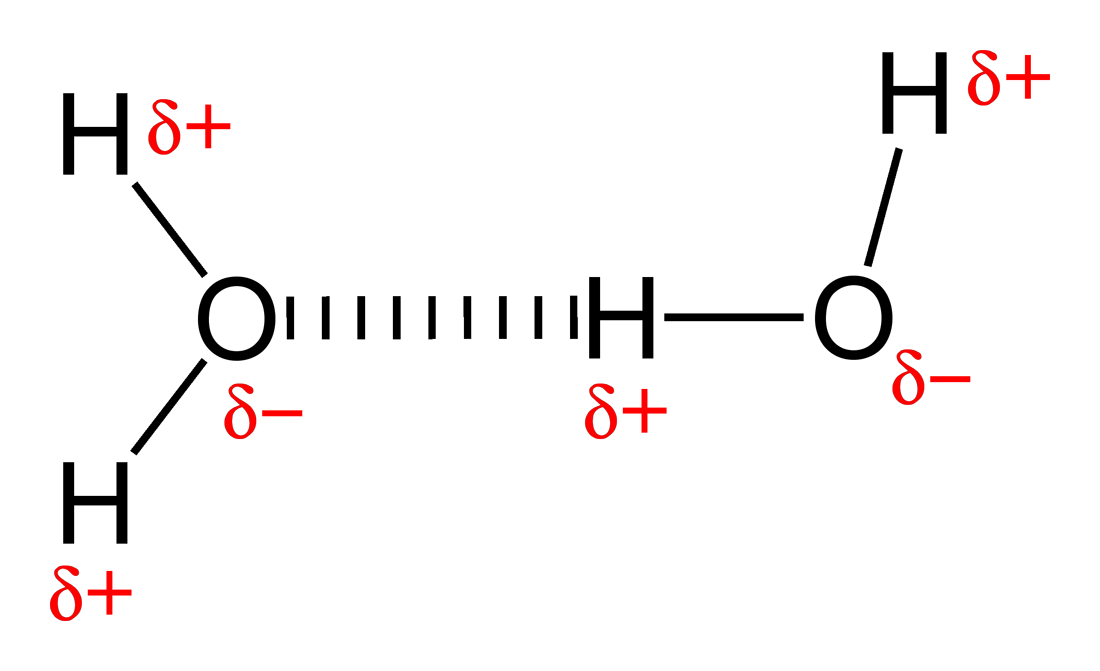
\includegraphics[scale=0.2]{Hydrogen-bonding-in-water-2D}
	\centering
	\caption{An example of hydrogen bonding in water. Image from wikipedia.}
\end{figure}

\end{document}
